\section{Componenti}

\subsection{PERCHÈ METTIAMO TUTTO INSIEME E DOPO COME SPLITTEREMO IN DUE}
qui spiega.

Ogni plugin per Kibana è articolato in due sezioni principali: lato client e lato server. Si presenta di seguito il dettaglio di ciasuna sezione.

\subsection{Lato Server}
Il lato server si deve occupare di interrogare il database Elasticsearch ed esporre i risultati delle query tramite API REST al lato client.
\subsubsection{Rappresentazione}
Nel seguente diagramma delle classi, figura \ref{img:diagrammaClassiServer}, ciascuna API viene rappresentata tramite una classe composta da un singolo metodo. Tale metodo intende rappresentare il funzionamento della API.


\begin{figure}[h]
	\centering
	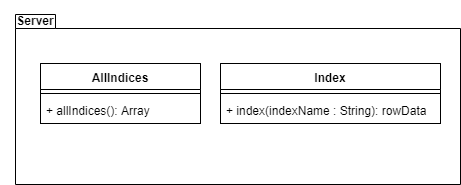
\includegraphics[width=1\textwidth]{Images/DiagrammaClassiServer.png}
	\caption{Diagramma UML delle classi riguardanti il lato server}
	\label{img:diagrammaClassiServer}
\end{figure}

\subsubsection{AllIndices}
AllIndices è la API che si occupa di restituire al chiamante la lista di \emph{tutti} gli indici presenti all'interno della istanza di Elasticsearch collegata. La lista degli indici è un array di stringhe contenente per ogni indice il proprio nome.

\subsubsection{Index}
Index è la API che espone l'interfaccia per poter leggere i dati contenuti all'interno di un indice. Nella richiesta GET deve essere specificato un parametro chiamato index, il cui valore rappresenta l'indice del quale si vogliono ottenere i dati. Ciò che viene ritornato al richiedente è un oggetto \emph{grezzo}, ovvero la risposta dell'istanza Elasticsearch, con tutti i metadati che Elasticsearch utilizza annessi. Sarà compito del client reperire le informazioni a lui utili

\subsection{Lato Client}
Il lato client si occupa di interrogare il lato server per ottenere informazioni grezze, elaborarle per renderle utili ed infine presentarle all'utente.

\label{sec:Componenti}
\subsubsection{Rappresentazione}
Il codice prodotto è stato scritto in Javascript ES6, quindi molti concetti quali classi ed interfacce non sono presenti all'interno del linguaggio. Per produrre un diagramma delle classi dunque sono state considerate \emph{ classi } sia oggetti Javascript, sia funzioni. Per quanto riguarda le interfacce che sono presenti nel diagramma delle classi \ref{diagrammaClassi}, nel codice non sono effettivamente presenti tali interfacce, ma tutte le classi che implementano tale interfaccia \emph{devono} possedere i metodi esposti da tale interfaccia.

\begin{figure}[H]
    \label{diagrammaClassi}
    \centering
    
\includegraphics[width=1\textwidth]{Images/logo.jpg}
    \caption{Diagramma delle classi dell'applicazione}
\end{figure}

\subsubsection{DataReader}
\label{sec:DataReader}
	\subsubsection{Diagramma}
	
	\subsubsection{Scopo}
	\texttt{DataReader} è il componente del sistema che si occupa di reperire i dati da ElasticSearch. Esso utilizza il metodo \texttt{setElasticsearchInstance(elastic)} per \textcolor{red}{qualcosa} e il metodo \texttt{readData()} per \textcolor{red}{qualcosaltro}.



\subsubsection{DataCleaner}
\label{sec:DataCleaner}
	\subsubsection{Diagramma}
	
	\subsubsection{Scopo}
	\texttt{DataCleaner} è il componente del sistema che si occupa di pulire i dati grezzi che sono stati reperiti da ElasticSearch. Esso compie questo lavoro in due tempi: prima estraendo i dati "utili" da ElasticSearch e poi pulendoli attraverso una strategy.\\
	Per estrarre i dati utili esso si avvale di un metodo, \texttt{removeMetaData(data)}, il quale si occupa di rimuovere i metadati di ElasticSearch che sono presenti quando si prelevano i dati. Questo metodo ritorna un array contenente i documenti JSON così come essi sono stati inseriti dall'applicazioni di monitoring negli indici di ElasticSearch. ElasticSearch, infatti, immagazzina i documenti JSON nel campo \texttt{\_source} il quale è inserito in oggetti che contengono altri dati ed informazioni "di servizio". Il metodo si occupa di rimuovere questi dati e costruisce un array contenente il solo contenuto dei campi \texttt{\_source}.\\
	Come secondo step, utilizzando il design pattern Strategy, esso si incarica di pulire i dati per la costruzione della Mappa Topologica oppure per la costruzione dello Stack Trace. \texttt{DataCleaner} contiene infatti un riferimento ad una strategia che al momento viene implementata in CleanerStrategy e GraphCleaner, anche se in futuro ne potrebbe essere implementata una diversa per svolgere compiti diversi. Le strategie contengono il metodo \texttt{clean(data)}, invocato passando i dati puliti da \texttt{removeMetaData()}. Tutto questo avviene nel metodo \texttt{cleanData()}.
	
\subsubsection{CleanerStrategy}
\label{sec:CleanerStrategy}
	\subsubsection{Diagramma}

	\subsubsection{Scopo}
	en do cazzo sta?
	
	
\subsubsection{GraphCleaner}
\label{sec:GraphCleaner}
	\subsubsection{Diagramma}

	\subsubsection{Scopo}
	\texttt{GraphCleaner} è l'implementazione della strategia utilizzata da \texttt{DataCleaner} per pulire i dati che dovranno essere utilizzati per la costruzione della mappa topologica. Essa dispone del metodo \texttt{clean(data)} il quale scorre tutti i documenti JSON \textcolor{red}{(specificare che sono usciti da removeMEtadata? e che contengono solo spans?)} disponibili e ha come output l'insieme di questi documenti che rappresentano chiamate a Database oppure a Server.
	
\subsubsection{StackCleaner}
\label{sec:StackCleaner}
	\subsubsection{Diagramma}
	
	\subsubsection{Scopo}
	\texttt{StackCleaner} è l'implementazione della strategia utilizzata da \texttt{DataCleaner} per pulire i dati che dovranno essere utilizzati per la costruzione della stack trace. Essa dispone del metodo \texttt{clean(data)} il quale scorre tutti i documenti JSON \textcolor{red}{stesse obiezioni di prima} disponibili e ha come output l'insieme di documenti che rappresentano chiamate HTTP, JDBC oppure Pageload \textcolor{red}{spiegare pageload}.
	

\subsubsection{StackBuilder}
\label{sec:StackBuilder}
	\subsubsection{Diagramma}

	\subsubsection{Scopo}
	\texttt{StackBuilder} si occupa della riorganizzazione dei dati e della loro sistemazione in modo da ottenere una struttura dati ottimale per la successiva costruzione della Stack Trace.\\
	Il metodo principale è \texttt{getStack()} che controlla tutte le chiamate HTTP ricevute da \texttt{StackCleaner()} e ne riorganizza i dati all'interno in base alla loro tipologia. Esse possono essere di tre tipi:
	\begin{itemize}
		\item HTTP: insieme di metodi scatenati da un'evento generico;
		\item HTTP + Pageload: insieme di metodi scatenati dal caricamento di una pagina web;
		\item HTTP + JDBC + Pageload: insieme di eventi che portano all''interrogazione di un database e che provocano un successivo caricamento di una pagina.
	\end{itemize}
	Per ognuna di questa tipologia è costruita una struttura dati che seleziona solo i campi del JSON ricevuto da \texttt{StackCleaner()} veramente utili alla generazione della stack trace. Per ognuna deve essere presente:
	\begin{itemize}
		\item \texttt{type}: che riconduce ad una delle tre tipologie di trace;
		\item \texttt{trace\_id}: numero univoco che permette l'associazione tra trace HTTP, JDBC e Pageload;
		\item \texttt{name}: identificazione generale della richiesta;
		\item \texttt{call\_tree}: array contenente gerarchicamente la lista dei metodi invocati dall'applicazione per compiere la richiesta;
		\item \texttt{duration}: tempo impiegato dal sistema per lo svolgimento della richiesta, compreso il tempo dei metodi, delle query e del caricamento della pagina;
		\item \texttt{timestamp}: data e ora dello svolgimento della richiesta;
		\item \texttt{error}: presenza o meno di errori;
		\item \texttt{status\_code}: tipologia di errore.
	\end{itemize}
	In particolare per il campo \texttt{call\_tree} avviene un'accurata manipolazione del dato attraverso i metodi \texttt{build\_tree()} e \texttt{tableTOtree()}. Al primo metodo viene  passato il dato sotto forma di stringa in cui, attraverso l'ASCII art, viene rappresentato un albero dei metodi che vengono invocati con delle informazioni particolari per ognuno di essi. Questo metodo costruisce un array bidimensionale che elenca tutti i metodi e per ognuno ne specifica i dati aggiuntivi rappresentati dall'ASCII art (come total time e self time), il grado di indentazione nell'albero, il numero di metodi figli e il numero di metodi discendenti da esso. \\ Da questa struttura il metodo \texttt{tableTOtree()} ricava un oggetto con innestati altri oggetti rappresentanti i metodi e i propri dati strutturati in maniera da rispecchiare i legami di parentela dell'ASCII art.
\subsubsection{GraphBuilder}
\label{sec:GraphBuilder}
	\subsubsection{Diagramma}

	\subsubsection{Scopo}
	\texttt{GraphBuilder} è la parte del sistema che si occupa di preparare i dati necessari per la costruzione della Mappa Topologica. In particolare utilizza i metodi \texttt{getNodes()} e \texttt{getLinks()} per riuscire a portare a termine il suo compito.\\
	Il metodo \texttt{getNodes()} costruisce l'insieme di nodi che faranno parte della mappa topologica. Esso scorre tutti i documenti JSON preparati dal \texttt{GraphCleaner()} e a seconda della tipologia della chiamata (a Database oppure a Server) crea un candidato ad entrare nella lista e attraverso il metodo \texttt{checkIfNotPresent()} si assicura che il candidato non sia già presente nella lista che verrà ritornata.\\
	Il metodo \texttt{getLinks()} invece costruisce l'insieme di collegamenti che ci saranno tra i nodi del grafo. Un link tra due nodi è caratterizzato dal campo \texttt{source}, il nodo che ha effettuato la chiamata, il campo \texttt{target}, quello che ha ricevuto la chiamata, il campo \texttt{type} che può essere "Database" o "Server",il campo \texttt{average\_response\_time} che contiene il tempo medio di risposta tra source e target e infine il campo \texttt{number\_of\_requests} che serve per tenere aggiornato il campo avg resp time. Ogni nodo è individuato univocamente dalla coppia \texttt{source} e \texttt{target}.\\	
	Per costruire l'insieme dei links \texttt{GraphBuilder} necessita sia della lista completa dei nodi sia dei dati puliti da \texttt{GraphCleaner}. Il metodo \texttt{getLinks()}, scorre tutti i dati e per ogni chiamata a database \textcolor{red}{DIRE CHE NON È ANCORA STATA IMPLEMENTATA LA COSA DI CHAIAMATE SERVER-SERVER?} e per ogni chiamata costruisce un candidato ad entrare nella lista. In seguito attraverso il metodo \texttt{checkIfLinkIsNotPresent()} viene controllato che la coppia source e target del candidato non sia già contenuta nella lista. Se essa non è contenuta il nuovo collegamento viene inserito, se invece è già contenuto si limita ad aggiornare i campi \texttt{average\_response\_time} e \texttt{number\_of\_requests}. \textcolor{red}{dire come è implementato aggiornamento del tempo medio magari}


\section{Interazioni fra componenti}
\label{sec:Interazioni}
Qui diagrammi di sequenza

\section{Tracciamento dei requisiti}
\label{sec:Tracciamento}
Qui swego 
